\clearpage

\begin{figure}[H]
\begin{center}
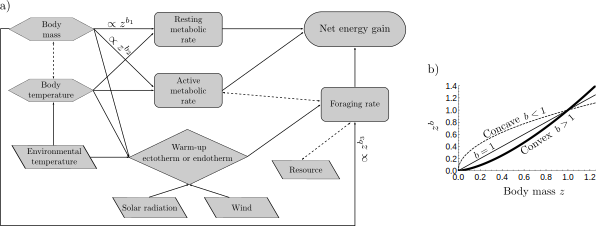
\includegraphics{fig1}
\caption{
    \setstretch{\stretchby}
    % E: For a figure to have multiple panels, the panels need to relate to one another.  Could (a) include, say, notes on the lines that depict power laws?
    Model components.
    (a) Unidirectional solid lines show one component affecting another.
    Bidirectional dashed lines show a correlation or indirect link between the two components.
    % E: Please also explain the different shapes used in (a), e.g., non-rhomboid parallelograms for environmental variables.
    (b) Power law functions of body size, $z$, are used throughout the model.
    The expression $z^b$ is concave when $0 < b < 1$ and convex when $b > 1$.
    % E: The caption and figure weren't agreeing before.  I changed in one way.  Please check!
}
\label{fig1}
\end{center}
\end{figure}

\clearpage

\begin{figure}[H]
\begin{center}
\includegraphics[width=\textwidth]{fig2}
\caption{
    \setstretch{\stretchby}
	Different scenarios where net energy gain peaks at intermediate body size as function of: resource quantity (a, b), resource quality (c, d), and metabolic cost (e, f, g, h) due to increase an in temperature and cost of activity.
	Thick, thin, and dashed lines are for $b_3 = 0.5, 0.8, \rm{ and }\, 1.25$, respectively.
	%
	Extrinsic parameters:
	For a) and b), high quantity $R = 500$ (an individual can collect at most 50 times its body mass), low quantity $R= 10$, resource quality $\rho = 12$, $T_e = 15$.
	For c) and d), high quality $\rho = 24$, low quality $\rho = 12$, total foraging time $\tau_f = 45 \rm{min}$, $T_e = 15$.
	For e) $T_e = 15$, for f) $T_e = 24.5$, $R = 500$, $\rho = 12$, and for g) $T_e = 17$
	Intrinsic parameters:
	For a), b), c), d), g), and h) $b_2 = 0.75, a_2 = 20 a_1$.
	For e) and f) we assumed a high active metabolic rate $a_2 = 30 a_1, b_2  = 1.25$.
	See \cref{table:table1} for units and default parameters.
}
\label{fig2}
\end{center}
\end{figure}

\begin{figure}[H]
\begin{center}
\scalebox{0.85}{\includegraphics{fig3}}
\caption{
    \setstretch{\stretchby}
	a) Lowest temperature required for the completion of warm-up as a function of body mass.
	The individual is given a maximum of 6 hours to complete warm-up.
	To show how solar radiation can limit warm-up, solar radiation at 30 degree latitude during equinox is scaled with a factor 0.25.
  Thick, thin, and dashed lines represent endotherms with laminar convection, ectotherms  with laminar convection, and ectotherms with free convection.
  Convection factor $K_2 = 0.1 \times$ the default value.
  b) Duration of warm-up for endotherms (thick lines) and ectotherms (dashed lines) as a function of body mass and temperature.
  In the scenario, solar radiation is not scaled and $K_2$ takes default values.
  Remaining parameters: wind speed  $u = 1$, $a_w = 1.25$.
	% Fixed parameter values: default conductance $K_1 = 0.05 \, c_p, r_3 = 0.5$.
	% Remaining parameters are in \cref{table:table1}.
	See \cref{table:table1} for units and default parameters.
}
\label{fig3}
\end{center}
\end{figure}
%
\begin{figure}[H]
\begin{center}
\scalebox{0.85}{\includegraphics{fig4}}
\caption{
    \setstretch{\stretchby}
Effect of warm-up on thermal performance for small (thin) and large (thick) body sizes ($z = 0.5 \mbox{ or } 2$) under free convection.
Warm-up starts half an hour after sunrise with a total foraging time $\tau_f = 1, \rho = 24, a_2 = 10 a_1, b_1 = b_2 = b_3 = 0.75.$
	See \cref{table:table1} for units and default parameters.
}
\label{fig4}
\end{center}
\end{figure}
\vspace{-0.8cm}
%\newpage
%%
\begin{figure}%[H]
\begin{center}
\scalebox{0.75}{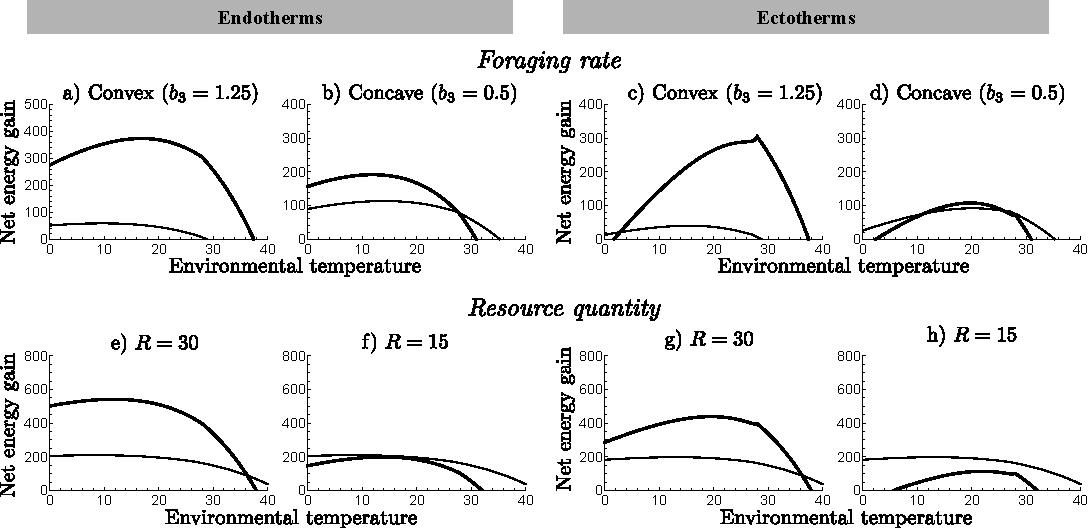
\includegraphics{fig5}}
\caption{
    \setstretch{\stretchby}
	Qualitative results on how foraging rate and resource quantity affect the thermal performance curves for small (thin) and large (thick) body sizes.
  We assumed free convection and warm-up starts half an hour after sunrise.
  For a--d, $\tau_f = 1$, ($z = 0.5 \mbox{ or } 2$) .
	For e--h, $b_1 = b_2 = b_3 = 0.75,$ ($z = 0.2 \mbox{ or } 2$)
	Remaining parameters: $\rho = 24, a_2 = 10 a_1$.
	See \cref{table:table1} for units and default parameters.
}
\label{fig5}
\end{center}
\end{figure}
